\documentclass[11pt,conference]{IEEEtran}

% IEEE standard packages
\usepackage{cite}
\usepackage{amsmath,amssymb,amsfonts}
\usepackage{algorithmic}
\usepackage{graphicx}
\usepackage{textcomp}
\usepackage{xcolor}

% Extra packages
\usepackage{booktabs} % For formal tables
\usepackage{xspace}
\usepackage{pete} % For Pete's annotations

% Writing helpers
\newcommand{\hc}{hierarchical consensus\xspace}
\newcommand{\Hc}{Hierarchical consensus\xspace}
\newcommand{\sub}{subquorum\xspace}
\newcommand{\Sub}{Subquorum\xspace}
\newcommand{\subs}{subquorums\xspace}
\newcommand{\Subs}{Subquorums\xspace}
\newcommand{\sys}{Alia\xspace}
\newcommand{\roo}{root quorum\xspace}
\newcommand{\roos}{root quorums\xspace}
\newcommand{\Roo}{Root quorum\xspace}
\newcommand{\Roos}{Root quorums\xspace}

\def\BibTeX{{\rm B\kern-.05em{\sc i\kern-.025em b}\kern-.08em
    T\kern-.1667em\lower.7ex\hbox{E}\kern-.125emX}}

\begin{document}

\title{Consensus Across Continents}

\author{
\IEEEauthorblockN{Benjamin Bengfort, Rebecca Bilbro, Pete Keleher}
\IEEEauthorblockA{Department of Computer Science\\
University of Maryland, College Park, MD, USA\\
\{bengfort,rbilbro,keleher\}@cs.umd.edu}}

\maketitle

\begin{abstract}
    Eventually consistent systems can be made more consistent by reducing the time
until a write is fully replicated, improving global visibility of updates.
While gossip-based anti-entropy methods scale well, random selection of
anti-entropy partners is less than efficient.
Moreover, while eventual consistency may be consistent enough in a single data
center, geographic replication increases visibility latency and leads to
externally observable inconsistencies.
In this paper, we explore an improvement to pairwise, bilateral anti-entropy;
instead of uniform random selection, we introduce reinforcement learning
mechanisms to assign selection probabilities to replicas most likely to have
information.
The result is more efficient replication, faster visibility, and stronger
eventual consistency while maintaining high availability and partition
tolerance.

\end{abstract}

\begin{IEEEkeywords}
hierarchical consensus, geographic replication, delegated voting, strong consistency
\end{IEEEkeywords}

\section{Introduction}
% The intro seems like a very good narrative and captures all of the moving pieces
% However, I'm worried that we're not getting across our awesome sauce soon enough (e.g. the first page)
% I'm also worried that we do not do enough to describe our system in a meaningful way
% Other papers like Akkio have 2 page intros though ...
% Just not sure how to do this narrative and lift things to the top
% To help this, I've added the system architecture diagram (fig 1) to the second page
% and referenced it, even though it's not considerded in detail until later in the paper -
% not totally sure if this is a good idea or not.

It is easier than ever before to deploy geographically distributed data systems
that span continents and oceans.
These types of systems leverage data centers newly available around the globe,
increasing local performance by minimizing network distance between users and
replicas, and offering data recovery in the face of catastrophes such as floods or
earthquakes.
Specialized, high-availability data systems~\cite{megastore,tao,akkio,dynamic_placement}
have maximized throughput across the wide area, driving interest in
geo-replicated systems and making truly international applications increasingly
feasible.
Managed replicated data services~\cite{spanner,aurora,cockroachdb} that can provide
strong consistency semantics for geographically distributed data systems have risen to
prominence.
However, while scalable consensus is effectively a solved problem, the solutions
introduced by these new systems and services require hardware and hardcoding that
inhibit change as system requirements change, e.g. as the userbase swells and becomes
increasingly multinational, as failures become more routine, and as user behaviors
become less geographically rooted.

Alia is the first distributed system of its kind to implement hierarchical consensus,
a flexible protocol that facilitates adaptation in geo-replicated distributed systems.
Hierarchical consensus comprises four key contributions; first, \emph{reconfigurable
consensus}, which allows systems to adapt to changing quorum membership, including
dynamic replacement and expansion; second, \emph{delegated voting}, which allows
decisions to be coordinated at the root (i.e. master) quorum, but executed by informed
hyperlocal subquora; third \emph{fuzzy transitions}, which allow the system to progress
unimpeded by leadership changes and reconfigurations; and finally, \emph{flexible data
placement}, which facilitates a greater proportion of direct accesses.
Together, these four features offer strong consistency at scale amidst dynamically
growing and shifting globally distributed systems of the kind required by modern
applications.

Traditional monolithic applications are being replaced by microservice
architectures and cloud-native service meshes~\cite{envoy} that make
infrastructure directly visible to applications.
As applications scale, service meshes make it easier to maintain and optimize
service-specific communication to minimize downtime and to improve system flexibility.
Additionally, due to increasing privacy regulation, application developers require more
control over data placement rather than less~\cite{gdpr}.
The engineering-based solutions of managed geo-distributed data services are designed to
coordinate hundreds of replicas that have access to expensive data-center hardware and
involves multiple, independent processes and quorums to synchronize time, allocate locks,
manage transations, and recover from failure.
Although these systems provide strong consistency, they do so in an rigid, opaque manner
that is not flexible enough for developers who require strong consistency at a higher
level of the application stack.

We propose a simpler approach to building large, geographically replicated systems.
Rather than relying on a fleet of loosely-coupled, independent small quorums whose
interactions are difficult to reason about, we propose a single, system-wide consensus
protocol that coordinates both replica placement and data accesses.
By ensuring that all coordination occurs through a single consensus activity,
it is easier to reason about the consistency of the system even in a network environment
prone to correlated failures, partitions, and variable latency.
Additionally, a single source of coordination gives the system the freedom to adapt to
changes in access patterns, configure to maximize throughput, specify data placement
rules, and ensure straightforward system maintenance.

In order to achieve this, a new consensus protocol that can scale beyond a handful of
replicas is required.
Distributed consensus, canonically represented by Paxos~\cite{paxos_simple} and its
performance optimizing
variants~\cite{fast_paxos,multicoordinated_paxos,spaxos,generalized_paxos}, primarily
consider safety in the case of one or two fail-stop node failures.
Although some recent research has explored the problem of geo-distributed
consensus~\cite{mencius,epaxos}, it primarily considers the problem of high-latency
links but geo-replication implies scale.
Services running around the globe recquire dozens if not hundreds of replicas and
introduce new failure modes such as network partitions, where sections of the system
operate independently without fail-stop failure, and highly variable latency that
inhibit quorum progress.
In order to scale systems beyond a handful of replicas, current
systems~\cite{spanner,scatter,mdcc,calvinfs} use Paxos as a component, instantiated
across multiple transactions, shards, or tablets to manage small subsystems
independently, leading to increased complexity and reduced transparency.

% the below paragraph needs help
We introduce a novel approach to scale consensus beyond a handful of nodes:
\emph{\hc}.
Our approach is to similarly decompose the consensus problem into units that can be
handled by provenly safe algorithms, but organizes all managed processes into an
intersecting hierarchy of quorums that ensure that all system-wide consensus decisions
are totally ordered.
The challenge is in building a multi-group coordination protocol that configures and
mediates \subs through a \roo.
The \roo guarantees correctness by pivoting the system through reconfigurations that
place replicas into \subs and maps them to partitions of the object namespace to handle
direct data accesses.

\ben{ended here}

% Contributions:
% - Reconfigurable consensus + adaptability
% - Delegated voting to scale consensus
% - Fuzzy transitions to allow progress
% - Access/policy optimized data placement rules


The \roo is composed of all replicas in the system, although reconfigurations are rare
with respect to data accesses, we introduce \emph{delegated voting} to optimize quorum
decisions at the root.

Much of the systems complexity comes from handshaking between the \roo and \subs during
reconfiguration.
These handshakes are made easier and far more efficient by using \emph{fuzzy transitions},
which allow individual \subs to move through reconfiguration at their own pace without

We validate our approach by implementing \hc in Alia, a linearizable object store
explicitly intended to run with many replicas, geo-replicated across heterogenous
networks and devices.
The resulting system is local, in that replicas serving clients can be located near them.
The system is fast because individual operations are served by a small group of replicas
regardless of the size of the total system.
The system is nimble in that it it can dynamically reconfigure the number, membership,
and responsibilities of the subquorums in response to failures, phase changes in the
driving applications or policy requirements for data placement and durability.
Finally, the system is consistent, supporting the strongest form of per-object
consistency without relying on special-purpose hardware.
We demonstrate its advantages through an implementation scaling to hundreds of replicas
across more than a dozen availability zones around the world using Amazon EC2.

% TODO: do we need rest of paper outline or contributions here?


\begin{figure}[t]
    \centering
    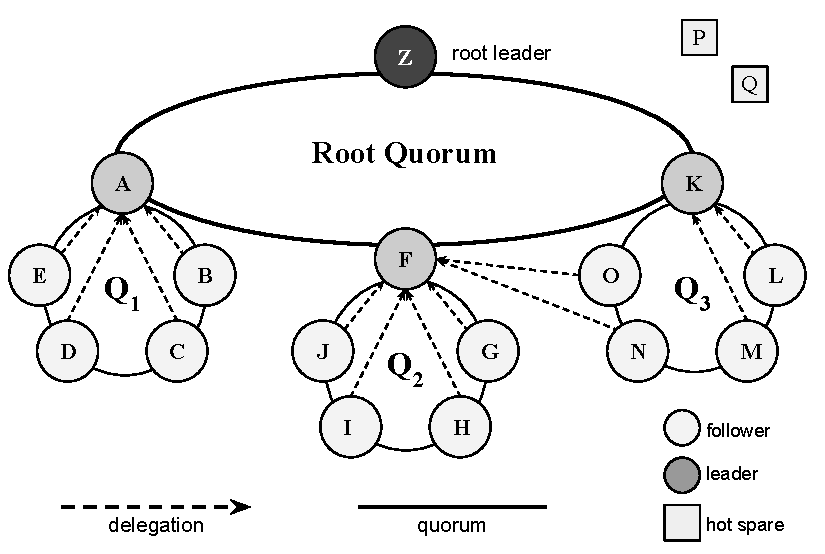
\includegraphics[width=0.5\textwidth]{figures/election3}
    \caption{Replicas participate in intersecting tiers of consensus.}
    \label{fig:system}
\end{figure}


\section{Conclusion}



Future work: investigate more tiers

\bibliographystyle{plain}
\bibliography{papers}

\end{document}